% Nama Kelompok 2 : Latitude & Longitude
% Kelas : D4TI3C
% Adhika Dwi Cahya Putra (1154017)
% Haris Munandar Alwi (1154105)
% Muhammad Adam Nahdlotul Halimi (1154024)
% Tito Aryo Nugroho (1154074)
% Tomy Prawoto (1154121)

\section{latitude longitude}

\subsection{Latitude}
Latitude merupakan terjemahan bahasa inggris dari garis lintang. Garis lintang dapat disebut juga sebagai garis khatulistiwa (0 derajat), atau bisa disebut juga sebagai garis tengah bumi yang membagi antara belahan bumi bagian atas dan bumi bagian bawah.
Dalam sebuah buku karangan Maling \& Derek Hylton yang berjudul \"Coordinate System and Map Projections\" mengatakan bahwa garis lintang suatu titik dapat didefinisikan secara formal sebagai sudut yang diukur di tengah bumi di antara bidang equator dan jari jari yang ditarik ke titik. 
Pada garis lintang bagian utara bumi dilambangkan dengan tanda \verb|'+phi'| 
sedangkan garis lintang bagian selatan bumi dilambangkan dengan tanda \verb|'-phi'| 
\cite{maling2013coordinate}. 

	\begin{figure}[ht]
	\centerline{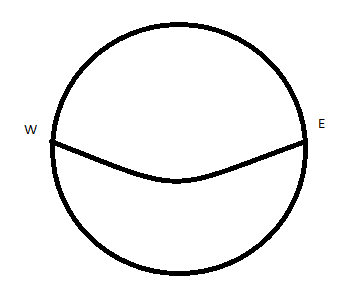
\includegraphics[width=1\textwidth]{figures/latitude.PNG}}
	\caption{Garis Lintang atau Latitude.}
	\label{latitude}
	\end{figure}
Pada gambar \ref{latitude} merupakan gambar latitude atau garis lintang yang membentang antara west(barat) sampai east(timur).
Garis lintang digunakan sebagai penanda dalam zona iklim di dunia. Dari +23 setengah derajat Lintang Utara sampai -23 setengah Lintang Selatan memiliki zona iklim tropis. Zona iklim tropis hanya memiliki dua musim, yaitu kemarau atau panas dan penghujan saja. Kemudian dari +23 setengah derajat Lintang utara sampai +66 setengah derajat Lintang utara memiliki zona iklim subtropis. Sama halnya bagian utara, bagian selatan yaitu -23 setengah derajat lintang selatan sampai -66 setengah derajat lintang selatan memiliki zona iklim subtropis. Daerah subtropis memiliki 4 musim, yaitu spring, summer, fall, dan winter. 

\subsection{Longitude}
Longitude merupakan terjemahan bahasa inggris dari garis bujur. Garis bujur biasa digunakan untuk menentukan waktu dan tanggal di dunia yang kita huni sekarang ini. Jika garis lintang atau latitude atau daerah khatulistiwa dianggap sebagai 0 derajat, maka garis bujur merupakan 0 derajat yang menghubungkan kutub utara dengan kutub selatan yang melawati kota Greenwich di Inggris. Garis bujur bagian barat kota Greenwich disebut sebagai Bujur Barat sedangkan garis bujur yang berada pada sebelah timur kota Greenwich disebut sebagai Bujur Timur. Inilah penyebab kenapa orang indonesia disebut sebagai orang timur.
	\begin{figure}[ht]
	\centerline{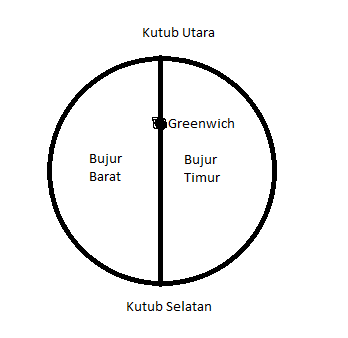
\includegraphics[width=1\textwidth]{figures/longitude.PNG}}
	\caption{Garis Bujur atau Longitude.}
	\label{longitude}
	\end{figure}
Pada gambar \ref{longitude} merupakan gambar longitude atau garis bujur yang menghubungkan kutub utara dengan kutub selatan. Garis ini melewati kota Greenwich di Inggris.
Garis bujur digunakan untuk pembagian zona waktu di dunia.

\section{LINTANG}

	Sudut lintang l
	Bayangkan Bumi adalah bola transparan (sebenarnya
	bentuknya agak oval; karena rotasi bumi, nya
	Khatulistiwa sedikit menonjol). Melalui Bumi yang transparan
	(gambar) kita bisa melihat bidang ekuatornya, dan bagian tengahnya
	titik adalah O, pusat bumi.
	Untuk menentukan garis lintang beberapa titik P di permukaan, tariklah
	radius OP ke titik itu. Maka sudut elevasi titik itu
	Di atas garis ekuator adalah garis lintang l - lintang utara jika utara
	dari garis khatulistiwa, lintang selatan (atau negatif) jika selatannya.
	Garis lintang. Di dunia bumi, garis lintang adalah lingkaran dengan ukuran yang berbeda. Itu
	terpanjang adalah khatulistiwa, yang garis lintangnya nol, sementara di kutub - di garis lintang
	90 ° utara dan 90 ° selatan (atau -90 °) lingkaran menyusut ke titik tertentu.

\section{GARIS BUJUR}
	Di dunia, garis bujur konstan ("meridian") meluas dari tiang ke kutub, seperti
	batas segmen pada jeruk kupas.
	Garis bujur atau "garis meridian"
	Setiap meridian harus melewati garis khatulistiwa. Karena ekuator adalah lingkaran, kita bisa
	bagilah itu - seperti lingkaran - ke dalam 360 derajat, dan bujur f dari sebuah titik adalah
	maka nilai yang ditandai dari divisi mana meridiannya memenuhi khatulistiwa.
	Apa nilai itu tergantung tentu saja dari mana kita mulai menghitung - di mana
	nol bujur adalah Untuk alasan historis, garis meridian melewati Astronomi Kerajaan yang lama
	Observatorium di Greenwich, Inggris, adalah yang dipilih sebagai nol bujur. Bertempat di Jl
	Tepi timur London, ibu kota Inggris, observatorium sekarang menjadi museum umum dan a
	band kuningan yang membentang di halamannya menandai "garis meridian utama". Wisatawan sering mendapatkan
	difoto saat mereka mengangkangnya - satu kaki di belahan bumi bagian timur, yang lainnya masuk belahan barat.
	Garis bujur juga disebut meridian, berasal dari bahasa Latin, dari meri, a
	variasi "medius" yang menunjukkan "tengah", dan diem, yang berarti "hari". Kata itu
	pernah berarti "siang", dan waktu sehari sebelum siang hari dikenal sebagai "ante meridian",
	sementara waktu setelah itu adalah "posting meridian." Singkatan hari ini a.m. dan p.m. datang
	Dari istilah ini, dan Matahari pada siang hari dikatakan "melewati meridian". Semua poin di
	garis bujur yang sama mengalami siang hari (dan jam lainnya) pada saat bersamaan dan
	oleh karena itu dikatakan sama "garis meridian", yang menjadi "meridian" untuk
	pendek.

\section{Waktu Lokal (LT) dan Zona Waktu}
	Garis bujur diukur dari nol sampai 180 ° BT dan 180 ° BB (atau -180 °), dan kedua 180-
	Gelombang longitudinal berbagi jalur yang sama, di tengah Samudera Pasifik.
	Saat Bumi berputar mengelilingi porosnya, kapanpun satu garis bujur - "siang hari
	meridian "- menghadap Matahari, dan pada saat itu, akan ada siang hari di mana-mana di atasnya
	jam Bumi telah mengalami rotasi penuh sehubungan dengan Matahari, dan meridian yang sama
	lagi wajah siang hari Jadi setiap jam Bumi berputar 360/24 = 15 derajat.
	Bila di lokasi Anda waktu 12 siang, 15 ° ke timur waktu adalah 1 p.m., karena itu adalah
	meridian yang dihadapi Matahari sejam yang lalu. Di sisi lain, 15 ° ke barat waktu adalah 11
	a.m., untuk satu jam lagi, meridian itu akan menghadapi Matahari dan mengalami siang hari.

\subsection{Glosarium}
	Khatulistiwa-Garis yang mengelilingi Bumi pada jarak yang sama dari Utara dan Selatan
	Polandia Koordinat geografis - Koordinat nilai yang diberikan sebagai garis lintang dan bujur.
	Lingkaran besar - Sebuah lingkaran terbentuk di permukaan bola oleh sebuah pesawat yang melewati
	pusat bola. Khatulistiwa, masing-masing meridian, dan satu sama lain keliling penuh
	Bumi membentuk lingkaran besar. Arus lingkaran besar menunjukkan jarak terpendek antara titik-titik di permukaan bumi.

	\subsubsection{Meridian}
	Lingkaran besar di permukaan Bumi, melewati kutub geografis
	dan beberapa titik ketiga di permukaan bumi. Semua poin pada meridian tertentu memiliki hal yang sama
	\subsubsection{Paralel}
	Lingkaran atau perkiraan lingkaran di permukaan Bumi, sejajar dengan
	Khatulistiwa dan titik penghubung dengan garis lintang yang sama.
	\subsubsection{Prime Meridian}
	Garis meridian bujur 0 derajat, digunakan sebagai asal untuk
	pengukuran bujur. Garis meridian Greenwich, Inggris, adalah internasional
	menerima meridian utama dalam banyak kasus.

\section{Konversi antara koordinat geografis dan cartesian koordinat}
	Asumsikan bahwa koordinat geografis dari suatu titik M adalah l dan f; asumsikan bahwa jari - jari
	Bumi adalah R. Masalahnya adalah penentuan koordinat kartesius M dalam a
	Sistem koordinat asal pusat bumi, dengan bidang horisontal xoy bidang
	Khatulistiwa, dengan sumbu x melewati meridian Greenwich, sumbu y secara langsung
	tegak lurus dengan sumbu x, dan akhirnya sumbu z melewati kutub.
	Tujuannya adalah untuk menemukan x, y dan z.

	Tunjukkan pada gambar sudut l dan f;
	Berapakah jarak OM?
	Hitung jarak OH menurut l.
	Berapakah nilai x dan y menurut l dan f;
	Berapakah nilai z?
	Asumsikan bahwa koordinat geografis dari suatu titik V
	adalah:
	garis lintang: 45 ° 41'47.59 '' N
	Bujur: 4 ° 52 '+ 49,98' 'E
	Apa koordinat kartesian V (dengan R = 1)
	Sebenarnya, titik ini persis sekolah kita!

\section{LINTANG/LATITUDE}

	Latitude adalah garis mendatar. Titik 0 adalah sudut ekuator tanda + menunjukan arah ke atas menuju kutub utara,
	sementara tanda minus di koordinat menuju ke kutub selatan. Bayangkan bila bumi hanyalah sebuah bola transparan 
	(sebenarnya bentuk bumi adalah oval; ini dikarenakan rotasi bumi itu sendiri, karena garis khatulistiwa sedikit 
	terlihat). Dengan bumi yang transparan, kita bisa lihat (gambar)
	\begin{figure}[ht]
	\centerline{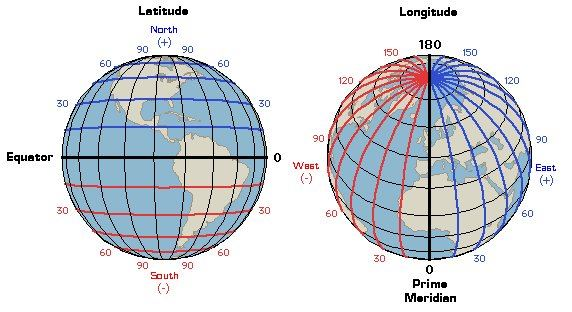
\includegraphics[width=1\textwidth]{figures/Latitude.jpg}}
	\caption{gambar Latitude.}
	\label{Gambar Latitude}
	\end{figure}
	garis khatulistiwa bumi, dan garis tengahnya adalah
	0, pusat bumi. Untuk menentukan latitude ( garis lintang ) dibeberapa titik P di permukaan, buatlah suatu jarak OP 
	ke suatu titik. Lalu sudut elevasi titik tersebut berada diatas garis ekuator adalah garis lintang l - lintang utara
	jika dari utara, lintang selatan ( negatif ) jika dari selatan. 
	Garis Lintang, dalam bola bumi, garis lintang dalam lingkaran memiliki perbedaan ukuran. Garis paling panjang adalah 
	Khatulistiwa, dimana yang lintangnya 0 ( nol ), sementara di daerah kutub, garis lintangnya 90° utara dan 90° selatan
	( atau bisa juga -90°) lingkarannya menyusut ke titik tertentu.

\section{BUJUR/LONGTITUDE}

	Longtitude adalah garis bujur, dimana garis bujur ini diawali dari titik 0° sampai 180° ke arah sebaliknya. Titik 0° dimulai dari
	garis negara Inggris, mengarah ke Indonesia akan menjadi angka positif. Jika koordinat longitude ( lintang ) akan menjadi minus 
	kearah kebalikan. Di bola bumi, garis bujur konstan meluas dari kutub ke kutub seperti batas segmen pada jeruk kupas. Garis Bujur atau
	Meridian ( gambar )
	\begin{figure}[ht]
	\centerline{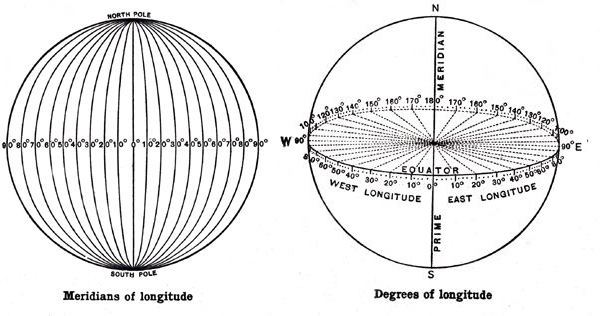
\includegraphics[width=1\textwidth]{figures/Longitude.jpg}}
	\caption{gambar longitude.}
	\label{Gambar Longitude}
	\end{figure}
	
	Setiap meridian harus menyberangi garis khatulistiwa. Karena khatulistiwa adalah sebuah lingkaran, kita bisa membagi nya seperti lingkaran
	yang lain ke dalam 360°,dan garis bujur f dari sebuah titik yang ditandai dimana meridian bertemu khatulistiwa.
	Nilai tersebut tentu bergantung pada saat kita mulai menghitung titik 0° garis bujur. Untuk alasan sejarah, garis bujur melewati Old Royal -
	Astronomical Obsevatory di Greenwich, Inggris, dimana garis 0° bujur di tetapkan. Berlokasi di tepi timur inggris, ibukota Inggris, Observatorium
	sekarang adalah Museum Umum dan suatu tanda yang membentang diatas halamannya yang menandai sebagai "garis meridian utama".
	Garis bujur atau dengan nama lain meridian, berasal dari bahasa latin, yaitu meri, variasi dari "merius" yang berarti "tengah" dan diem yang berarti 
	"hari". Kata tersebut juga bisa berarti "sore", dan waktu pada satu hari sebelum sore kita sebut sebagai "ante meridian" dimana waktu setelahnya berarti 
	"post meridian".Pada saat ini disingkat menjadi a.m. dan p.m. yang berasal dari istilah ini, dan matahari pada saat menjelang malam hari disebut sebagai
	"passing meridians". Semua titik pada setiap garis yang sama dalam garis bujur disebut sore ( dan pada jam lainnya ) pada saat yang sama dan oleh karena 
	itu disebut "garis meridian", yang menjadi "meridian" untuk lebih singkat.
